% ─────────────────────────────────────────────────────────────
% CHAPTER 4: SYSTEM ARCHITECTURE & REQUIREMENTS ANALYSIS
% ─────────────────────────────────────────────────────────────
\chapter{System Architecture \& Requirements Analysis}
\label{ch:system_architecture}

\section{Requirement Gathering and Engineering Analysis}
\label{sec:arch_requirements}

Before engineering production backend services, thorough systems analysis was conducted in collaboration with Digicon's business analysts, BPO team leads, and lead software architects. The objective was to specify exact functional deliverables and non-functional performance guarantees for two core enterprise modules: the \textbf{Customer Relationship Management (CRM) Support Ticket Routing Engine} and the \textbf{Enterprise SMS Gateway Microservice}.

\subsection{Functional Requirements (FR)}
The functional specifications define the operational capabilities that the backend systems must execute:

\begin{enumerate}
    \item \textbf{User Management and Access Control (FR-01):}
    \begin{itemize}
        \item Secure authentication via email and salted/hashed passwords.
        \item Issuance of cryptographically signed JWT access tokens and HTTP-only refresh tokens.
        \item Enforcement of Role-Based Access Control (RBAC) permitting distinct administrative operations across SuperAdmin, TeamLead, SupportAgent, and Customer roles.
    \end{itemize}
    \item \textbf{CRM Ticket Management and SLA Lifecycle (FR-02):}
    \begin{itemize}
        \item Ingestion of support tickets generated from multi-channel inputs (telephony calls, web forms, email, and social media webhooks).
        \item Dynamic assignment of priority tiers (\texttt{LOW}, \texttt{MEDIUM}, \texttt{HIGH}, \texttt{CRITICAL}) and automated calculation of Service Level Agreement (SLA) breach timestamps.
        \item Intelligent agent skill-matching and ticket assignment based on real-time agent presence tracked in Redis.
        \item State transition management (\texttt{OPEN} $\to$ \texttt{IN\_PROGRESS} $\to$ \texttt{ESCALATED} $\to$ \texttt{RESOLVED} $\to$ \texttt{CLOSED}) with mandatory immutable audit logging.
    \end{itemize}
    \item \textbf{Enterprise SMS Gateway and Batch Queuing (FR-03):}
    \begin{itemize}
        \item Ingestion of single and bulk SMS dispatch requests via authenticated REST endpoints.
        \item Dynamic phone number normalization and telecommunication carrier identification (Grameenphone, Robi, Banglalink, Teletalk).
        \item Asynchronous queuing of dispatch jobs into Redis BullMQ to decouple client HTTP requests from carrier dispatch latency.
        \item Webhook callback receiver to ingest real-time Delivery Receipts (DLR) from telecom aggregators, with cryptographic verification of payload signatures.
    \end{itemize}
\end{enumerate}

\subsection{Non-Functional Requirements (NFR)}
Non-functional requirements establish the qualitative and architectural constraints under which the systems must operate:

\begin{itemize}
    \item \textbf{High Concurrency and Scalability (NFR-01):} The backend infrastructure must support over 1,500 active concurrent contact center agents without thread starvation. The SMS gateway must handle sustained throughput exceeding 1,500 messages per second.
    \item \textbf{Low Latency (NFR-02):} Core API endpoints must respond with sub-50ms latency for 95\% of requests under normal load, achieved through multi-tier Redis caching.
    \item \textbf{High Availability and Fault Tolerance (NFR-03):} Maintain 99.98\% operational uptime. Outbound telecom failures must not result in message loss; the queue must execute automated exponential backoff retries.
    \item \textbf{Data Integrity and Consistency (NFR-04):} Ticket assignments must employ optimistic concurrency control to prevent multiple agents from simultaneously locking or mutating the same ticket document.
    \item \textbf{Security and Regulatory Compliance (NFR-05):} Complete adherence to OWASP Top 10 guidelines, TLS 1.3 transport encryption, and compliance with the Bangladesh Telecommunication Regulatory Commission (BTRC) messaging guidelines.
\end{itemize}

\section{High-Level Layered Microservices Architecture}
\label{sec:arch_layered}

To satisfy both functional flexibility and enterprise scalability, the backend system was architected following the \textbf{Multi-Tier Layered Architecture} and the \textbf{Microservices Pattern} \citep{newman2021building}. Figure~\ref{fig:backend_layered_architecture} delineates the comprehensive six-layer architectural blueprint.

\begin{figure}[htbp]
    \centering
    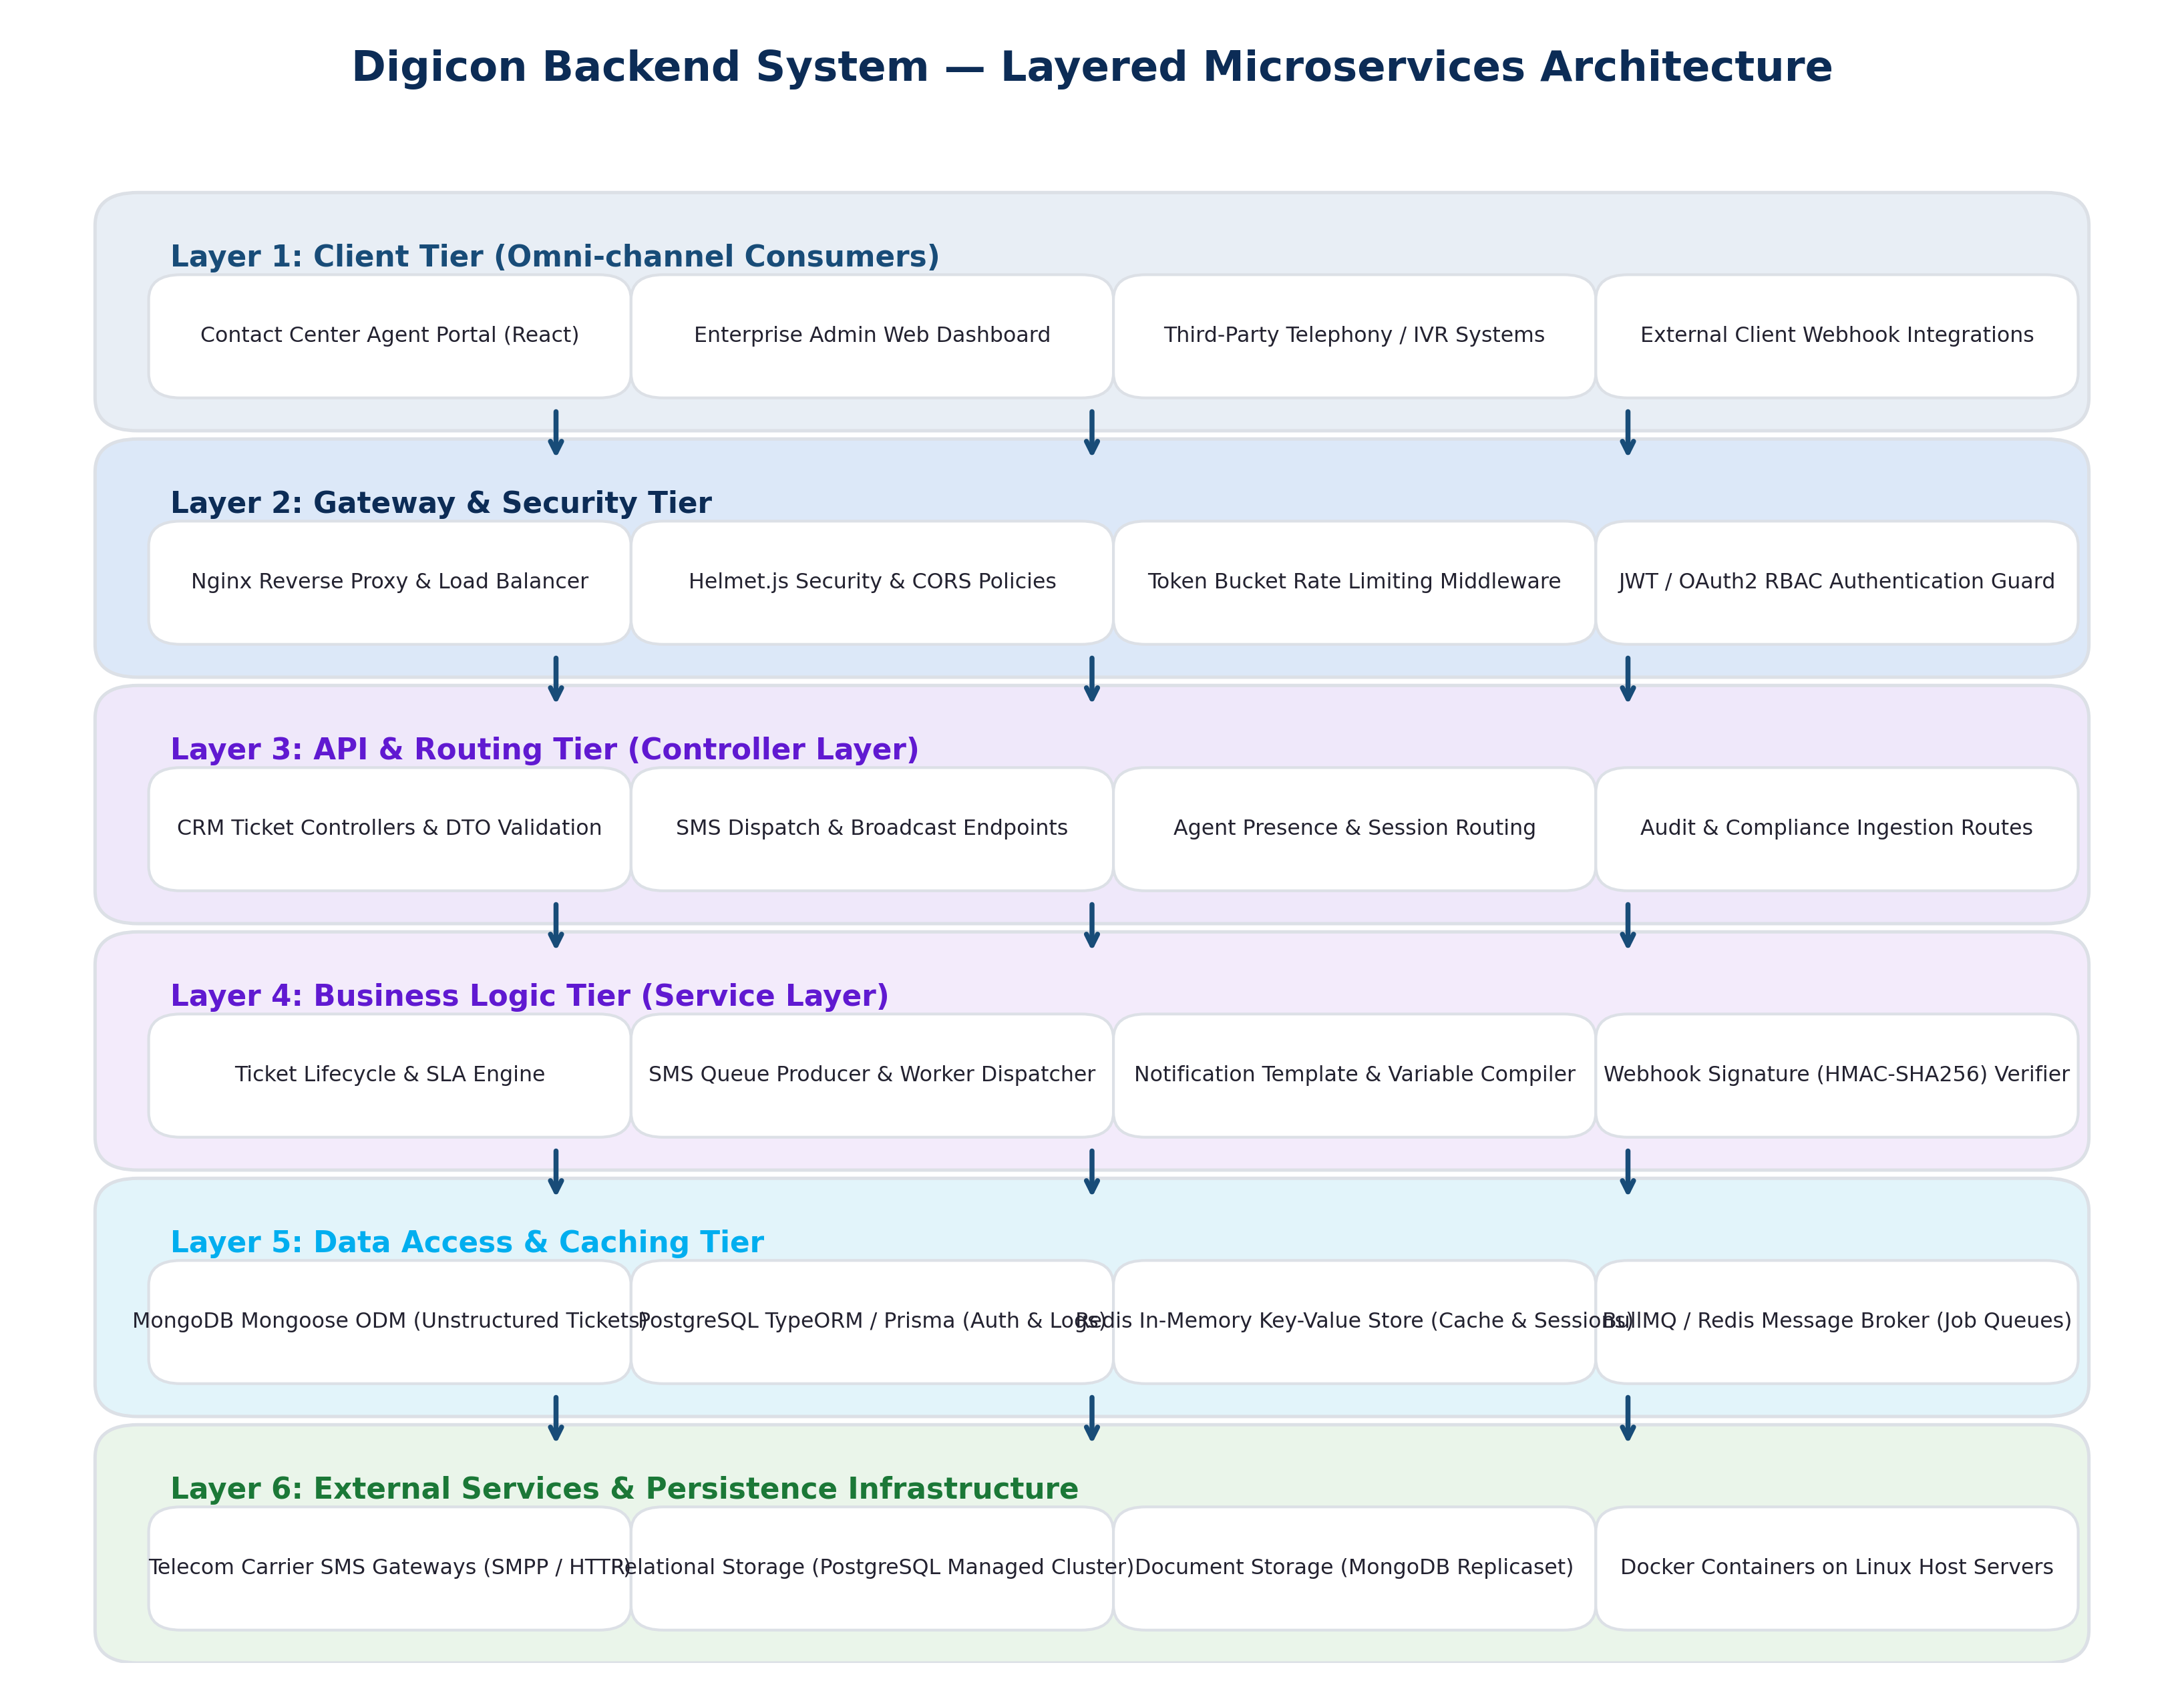
\includegraphics[width=0.95\textwidth]{figures/backend_layered_architecture.png}
    \caption{Digicon Backend System — Layered Microservices Architecture.}
    \label{fig:backend_layered_architecture}
\end{figure}

The architecture is partitioned into cleanly decoupled tiers:
\begin{enumerate}
    \item \textbf{Client Tier:} Represents diverse omni-channel consumers, including the React-based Contact Center Agent Workspace, administrative dashboards, automated IVR telephony servers, and external third-party webhook integrations.
    \item \textbf{Gateway \& Security Tier:} The entry point for all external traffic. \textbf{Nginx} acts as a reverse proxy, terminating SSL/TLS certificates and distributing traffic across clustered Node.js worker processes. \textbf{Helmet.js} and CORS middleware enforce transport security, while a \textbf{Token Bucket Rate Limiter} defends against denial-of-service spikes. An authorization guard verifies JWT signatures before requests enter application memory.
    \item \textbf{API \& Routing Tier (Controllers):} Implemented using NestJS and Express routers. Controllers are strictly responsible for route binding, parsing URL parameters, executing declarative DTO payload validation via \texttt{class-validator}, and delegating tasks to underlying services.
    \item \textbf{Business Logic Tier (Services):} Contains domain business rules isolated from HTTP transport mechanics. The \textit{Ticket Service} evaluates SLA timers, determines agent availability, and manages status transitions. The \textit{SMS Dispatcher Service} compiles dynamic templates and produces jobs for asynchronous queue workers.
    \item \textbf{Data Access \& Caching Tier:} Encapsulates persistence logic. The \textit{Mongoose ODM} interfaces with MongoDB for unstructured ticket documents. \textit{Prisma / TypeORM} executes relational queries against PostgreSQL for user identities and audit logs. The \textit{Redis Layer} serves a dual role: caching frequently read entities and powering the \textit{BullMQ} distributed message broker.
    \item \textbf{External Infrastructure Tier:} Comprises underlying bare-metal Linux servers executing containerized Docker workloads, managed PostgreSQL/MongoDB database clusters, and external telecommunication carrier SMPP/HTTP endpoints.
\end{enumerate}

\section{Database Schema and Data Modeling}
\label{sec:arch_db_schema}

The polyglot persistence strategy adopted at Digicon strategically segregates structured transactional entities from flexible document entities. Figure~\ref{fig:database_er_schema} presents the database Entity-Relationship and document schema architecture.

\begin{figure}[htbp]
    \centering
    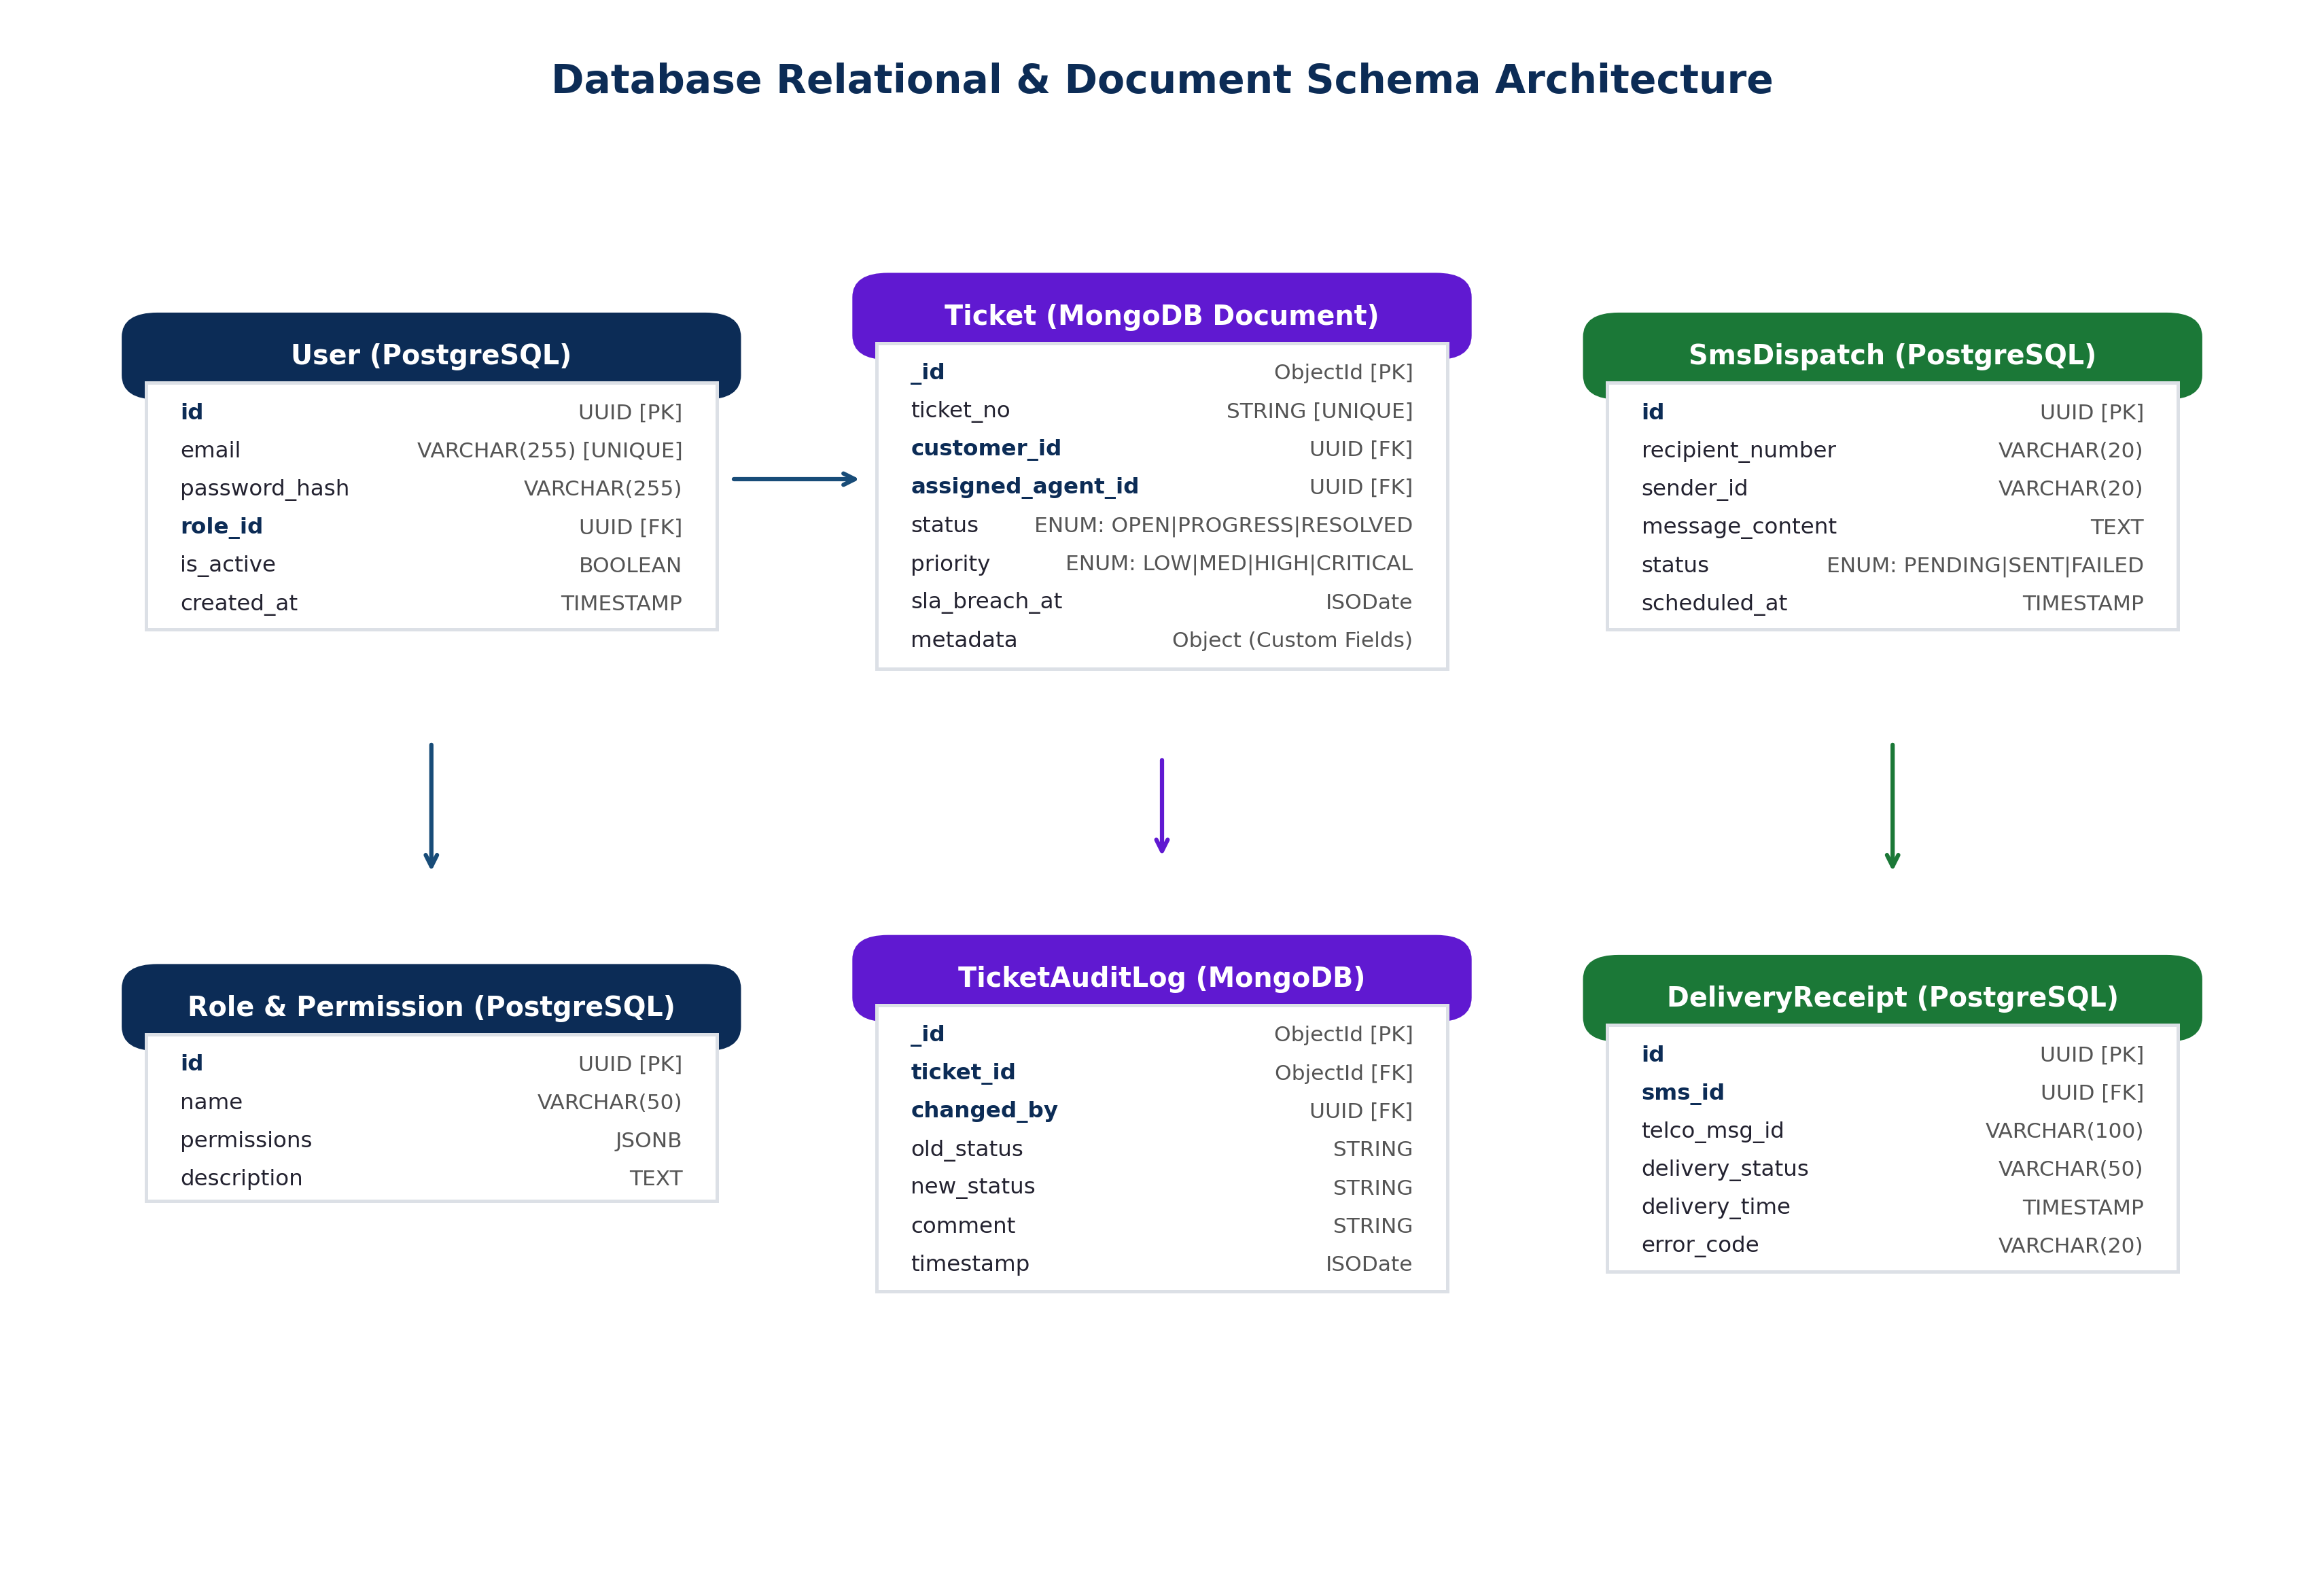
\includegraphics[width=0.95\textwidth]{figures/database_er_schema.png}
    \caption{Database Relational and Document Schema Architecture.}
    \label{fig:database_er_schema}
\end{figure}

\subsection{Relational PostgreSQL Entities}
\begin{itemize}
    \item \textbf{User Table:} Stores system operators and contact center staff. Employs a \texttt{UUID} primary key, unique email index, Bcrypt hashed password, foreign key reference to the \texttt{Role} entity, and account activation flags.
    \item \textbf{Role \& Permission Table:} Defines granular authorization roles. The \texttt{permissions} attribute is modeled as a PostgreSQL \texttt{JSONB} field, permitting high-speed indexed lookups of specific capability flags (e.g., \texttt{\{"tickets": ["read", "write", "escalate"]\}}).
    \item \textbf{SmsDispatch Table:} Records every outbound SMS transmission with unique tracking UUIDs, recipient phone number, alphanumeric sender ID, message body, current status (\texttt{PENDING}, \texttt{SENT}, \texttt{FAILED}), and scheduling timestamps.
    \item \textbf{DeliveryReceipt Table:} Persists telecommunication carrier delivery reports (DLR). Relates to \texttt{SmsDispatch} via a foreign key, recording the carrier's internal message ID, final delivery state (\texttt{DELIVRD}, \texttt{UNDELIV}, \texttt{EXPIRED}), delivery timestamp, and error diagnostics.
\end{itemize}

\subsection{Document MongoDB Entities}
\begin{itemize}
    \item \textbf{Ticket Collection:} Represents customer support cases. Modeled as a MongoDB document containing unique ticket numbers, customer identifiers, assigned agent IDs, categorical status enums, priority rankings, calculated SLA breach timestamps, and a dynamic \texttt{metadata} subdocument accommodating custom client-specific fields. Compound indexes are constructed on \texttt{\{status: 1, priority: -1, sla\_breach\_at: 1\}} to ensure sub-millisecond query execution during queue sorting.
    \item \textbf{TicketAuditLog Collection:} An immutable, append-only collection that captures every state alteration, recording the acting user ID, old status, new status, explanatory comment, and exact ISO timestamp, satisfying strict corporate compliance auditing.
\end{itemize}

\section{CRM Ticket Lifecycle and Event Routing Flow}
\label{sec:arch_crm_flow}

The lifecycle of a customer support ticket within Digicon's contact center involves intricate orchestration across HTTP routes, database transactions, caching layers, and WebSocket event emitters. Figure~\ref{fig:crm_ticket_flow} visualizes the complete end-to-end lifecycle progression.

\begin{figure}[htbp]
    \centering
    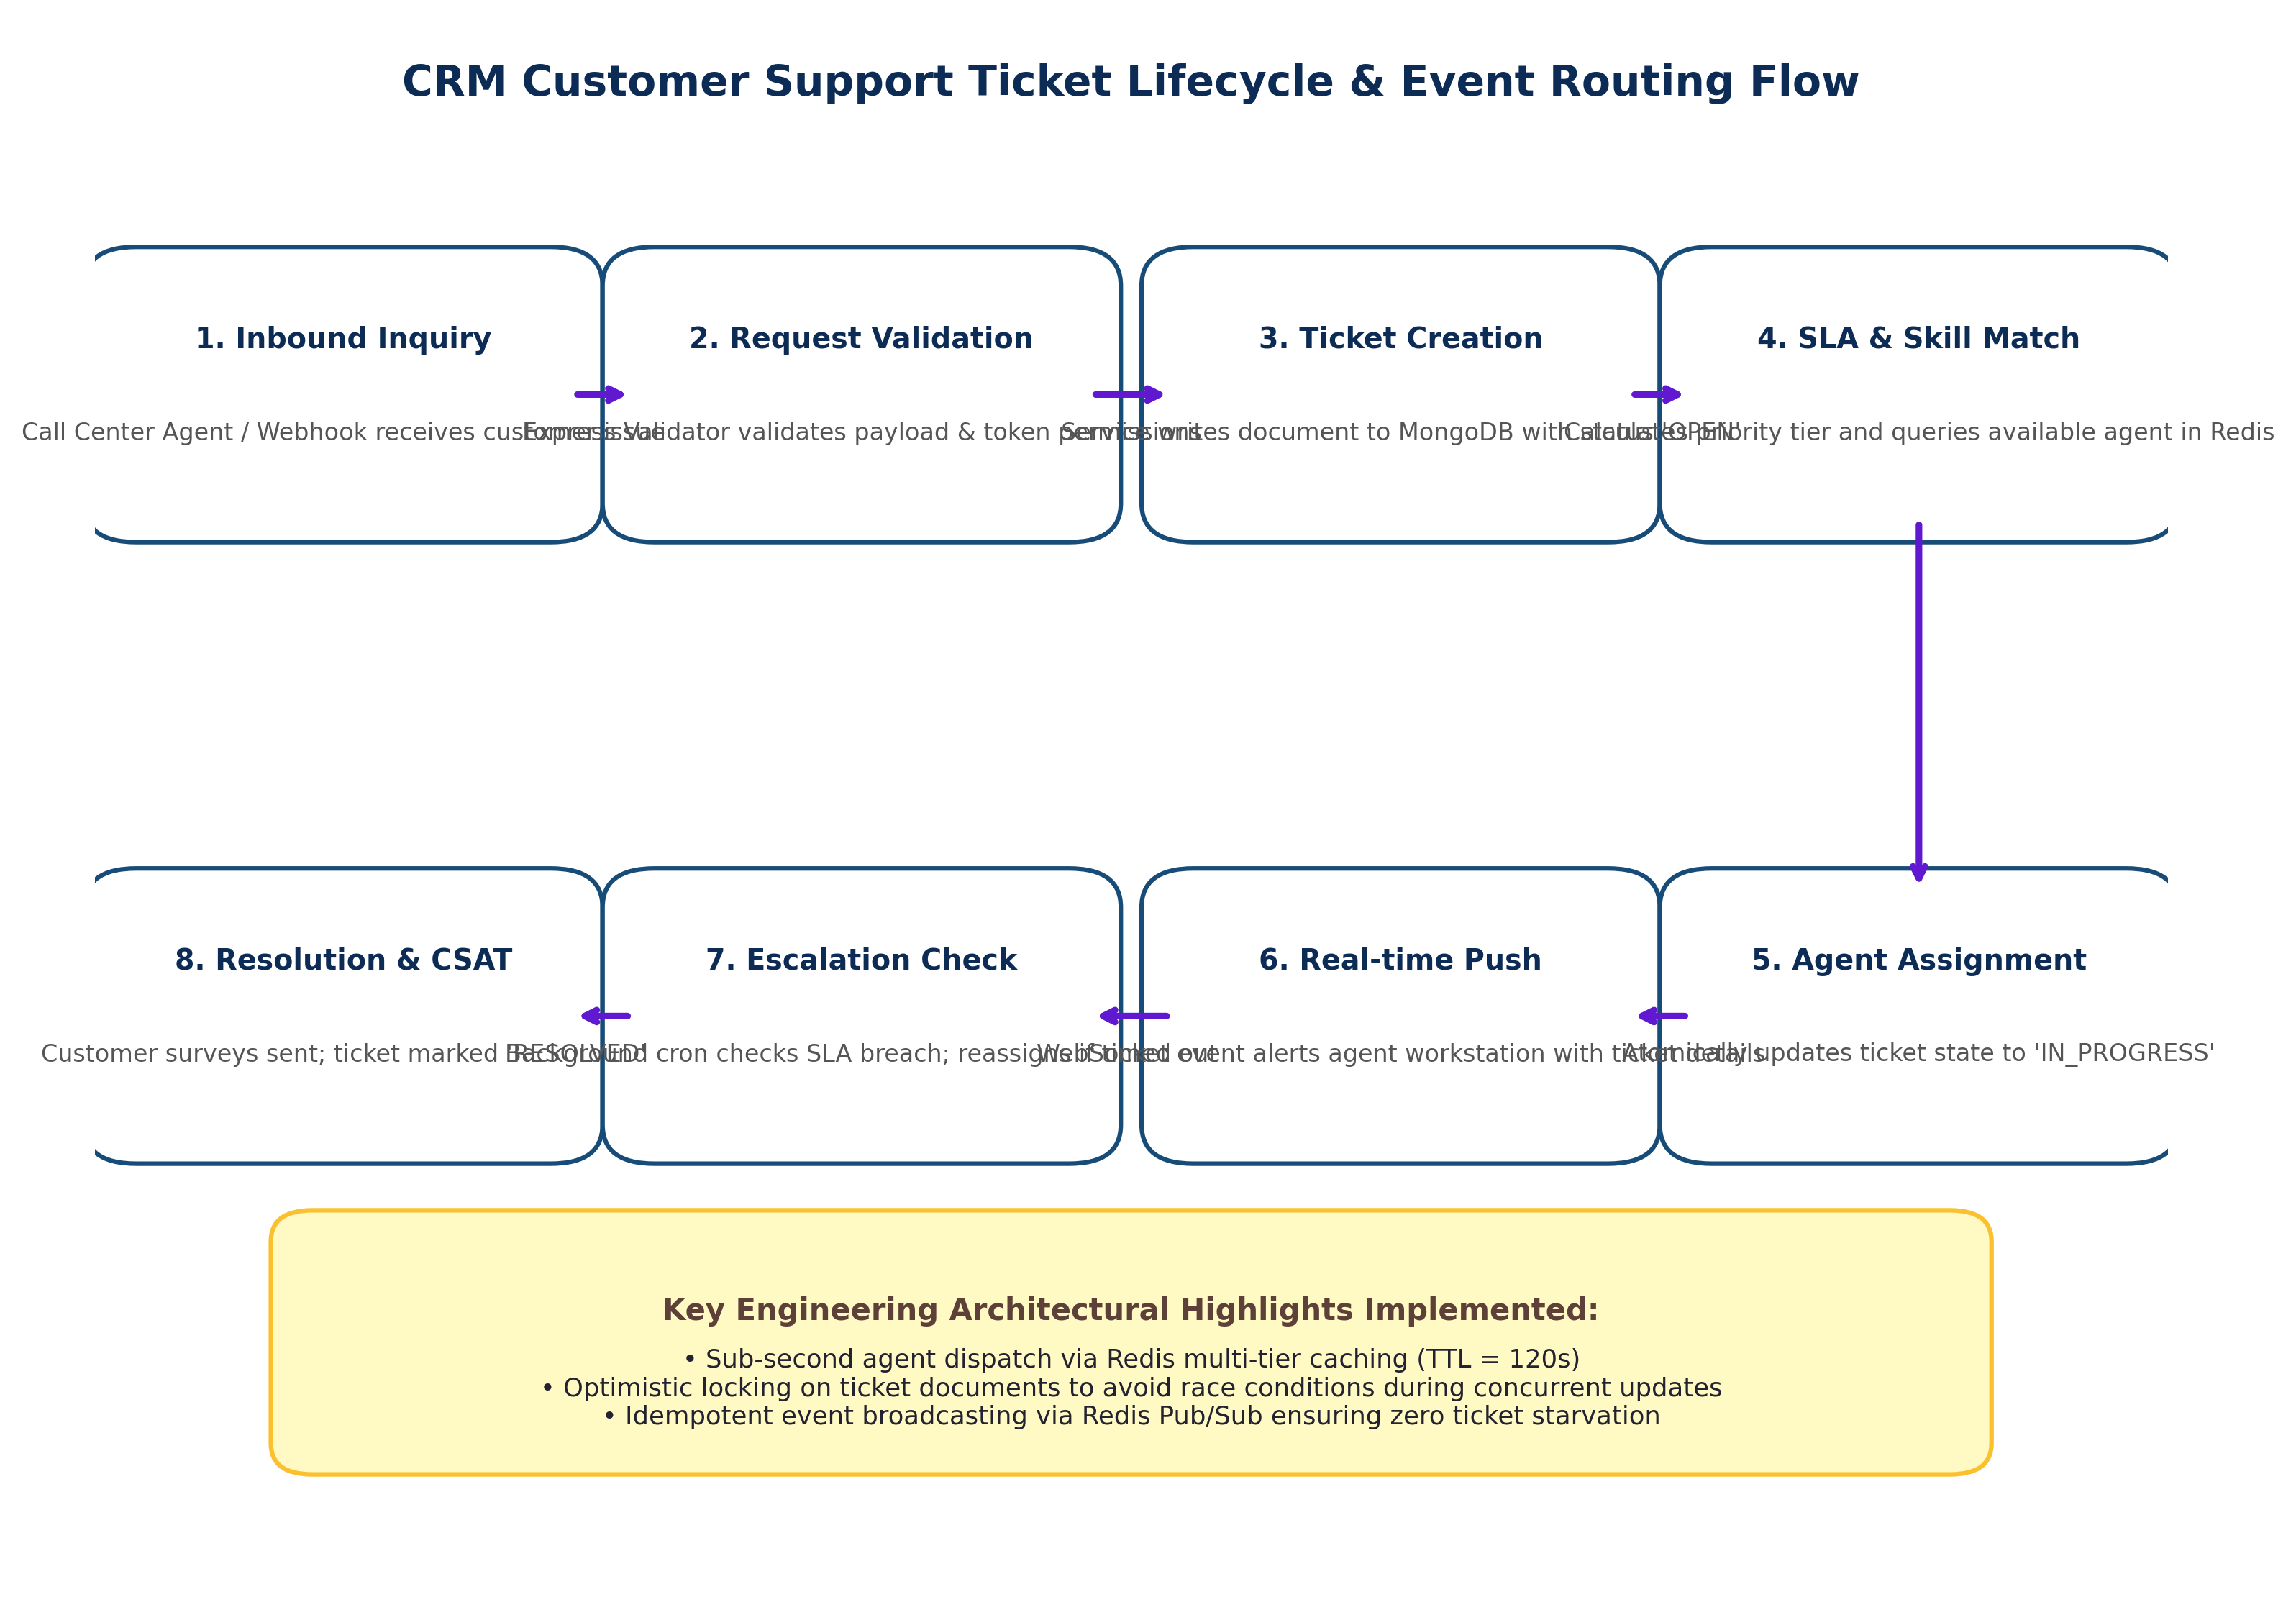
\includegraphics[width=0.95\textwidth]{figures/crm_ticket_flow.png}
    \caption{CRM Customer Support Ticket Lifecycle and Event Routing Flow.}
    \label{fig:crm_ticket_flow}
\end{figure}

The sequential flow operates through eight clearly defined stages:
\begin{enumerate}
    \item \textbf{Inbound Inquiry Ingestion:} Inbound customer communications arriving from call center telephony, web forms, or external client webhooks trigger a \texttt{POST /api/v1/tickets} invocation.
    \item \textbf{Payload Validation:} Express Validator and DTO pipes verify that mandatory fields (customer ID, issue category, description) conform to data schemas and that the client's JWT possesses \texttt{TICKET\_CREATE} privileges.
    \item \textbf{Document Creation:} The ticket is written to MongoDB with initial status \texttt{OPEN}.
    \item \textbf{SLA Calculation \& Skill Matching:} The service calculates the maximum allowable resolution window based on customer contract tier (e.g., Critical = 2 hours, Low = 24 hours). Concurrently, an in-memory Redis query identifies currently active, non-overloaded agents matching the required skill domain.
    \item \textbf{Atomic Agent Assignment:} The ticket document is updated with the assigned agent ID and status transitioned to \texttt{IN\_PROGRESS} using optimistic locking to prevent double-assignment.
    \item \textbf{Real-Time WebSocket Push:} A Redis Pub/Sub event is emitted, causing the WebSocket gateway to push the new ticket notification directly to the selected agent's browser workstation within 50 milliseconds.
    \item \textbf{Escalation Daemon Monitoring:} A scheduled background cron evaluates tickets approaching SLA breach, automatically raising priority and alerting team leads if resolution thresholds are crossed.
    \item \textbf{Resolution and Feedback:} Upon problem resolution, the agent updates the status to \texttt{RESOLVED}. An automated SMS notification containing a CSAT rating link is enqueued to the customer.
\end{enumerate}

\section{Enterprise SMS Gateway and Asynchronous Queue Architecture}
\label{sec:arch_sms_pipeline}

The SMS Gateway microservice was designed to address high-volume message delivery under strict telecom rate constraints. Figure~\ref{fig:sms_gateway_pipeline} illustrates the asynchronous pipeline architecture.

\begin{figure}[htbp]
    \centering
    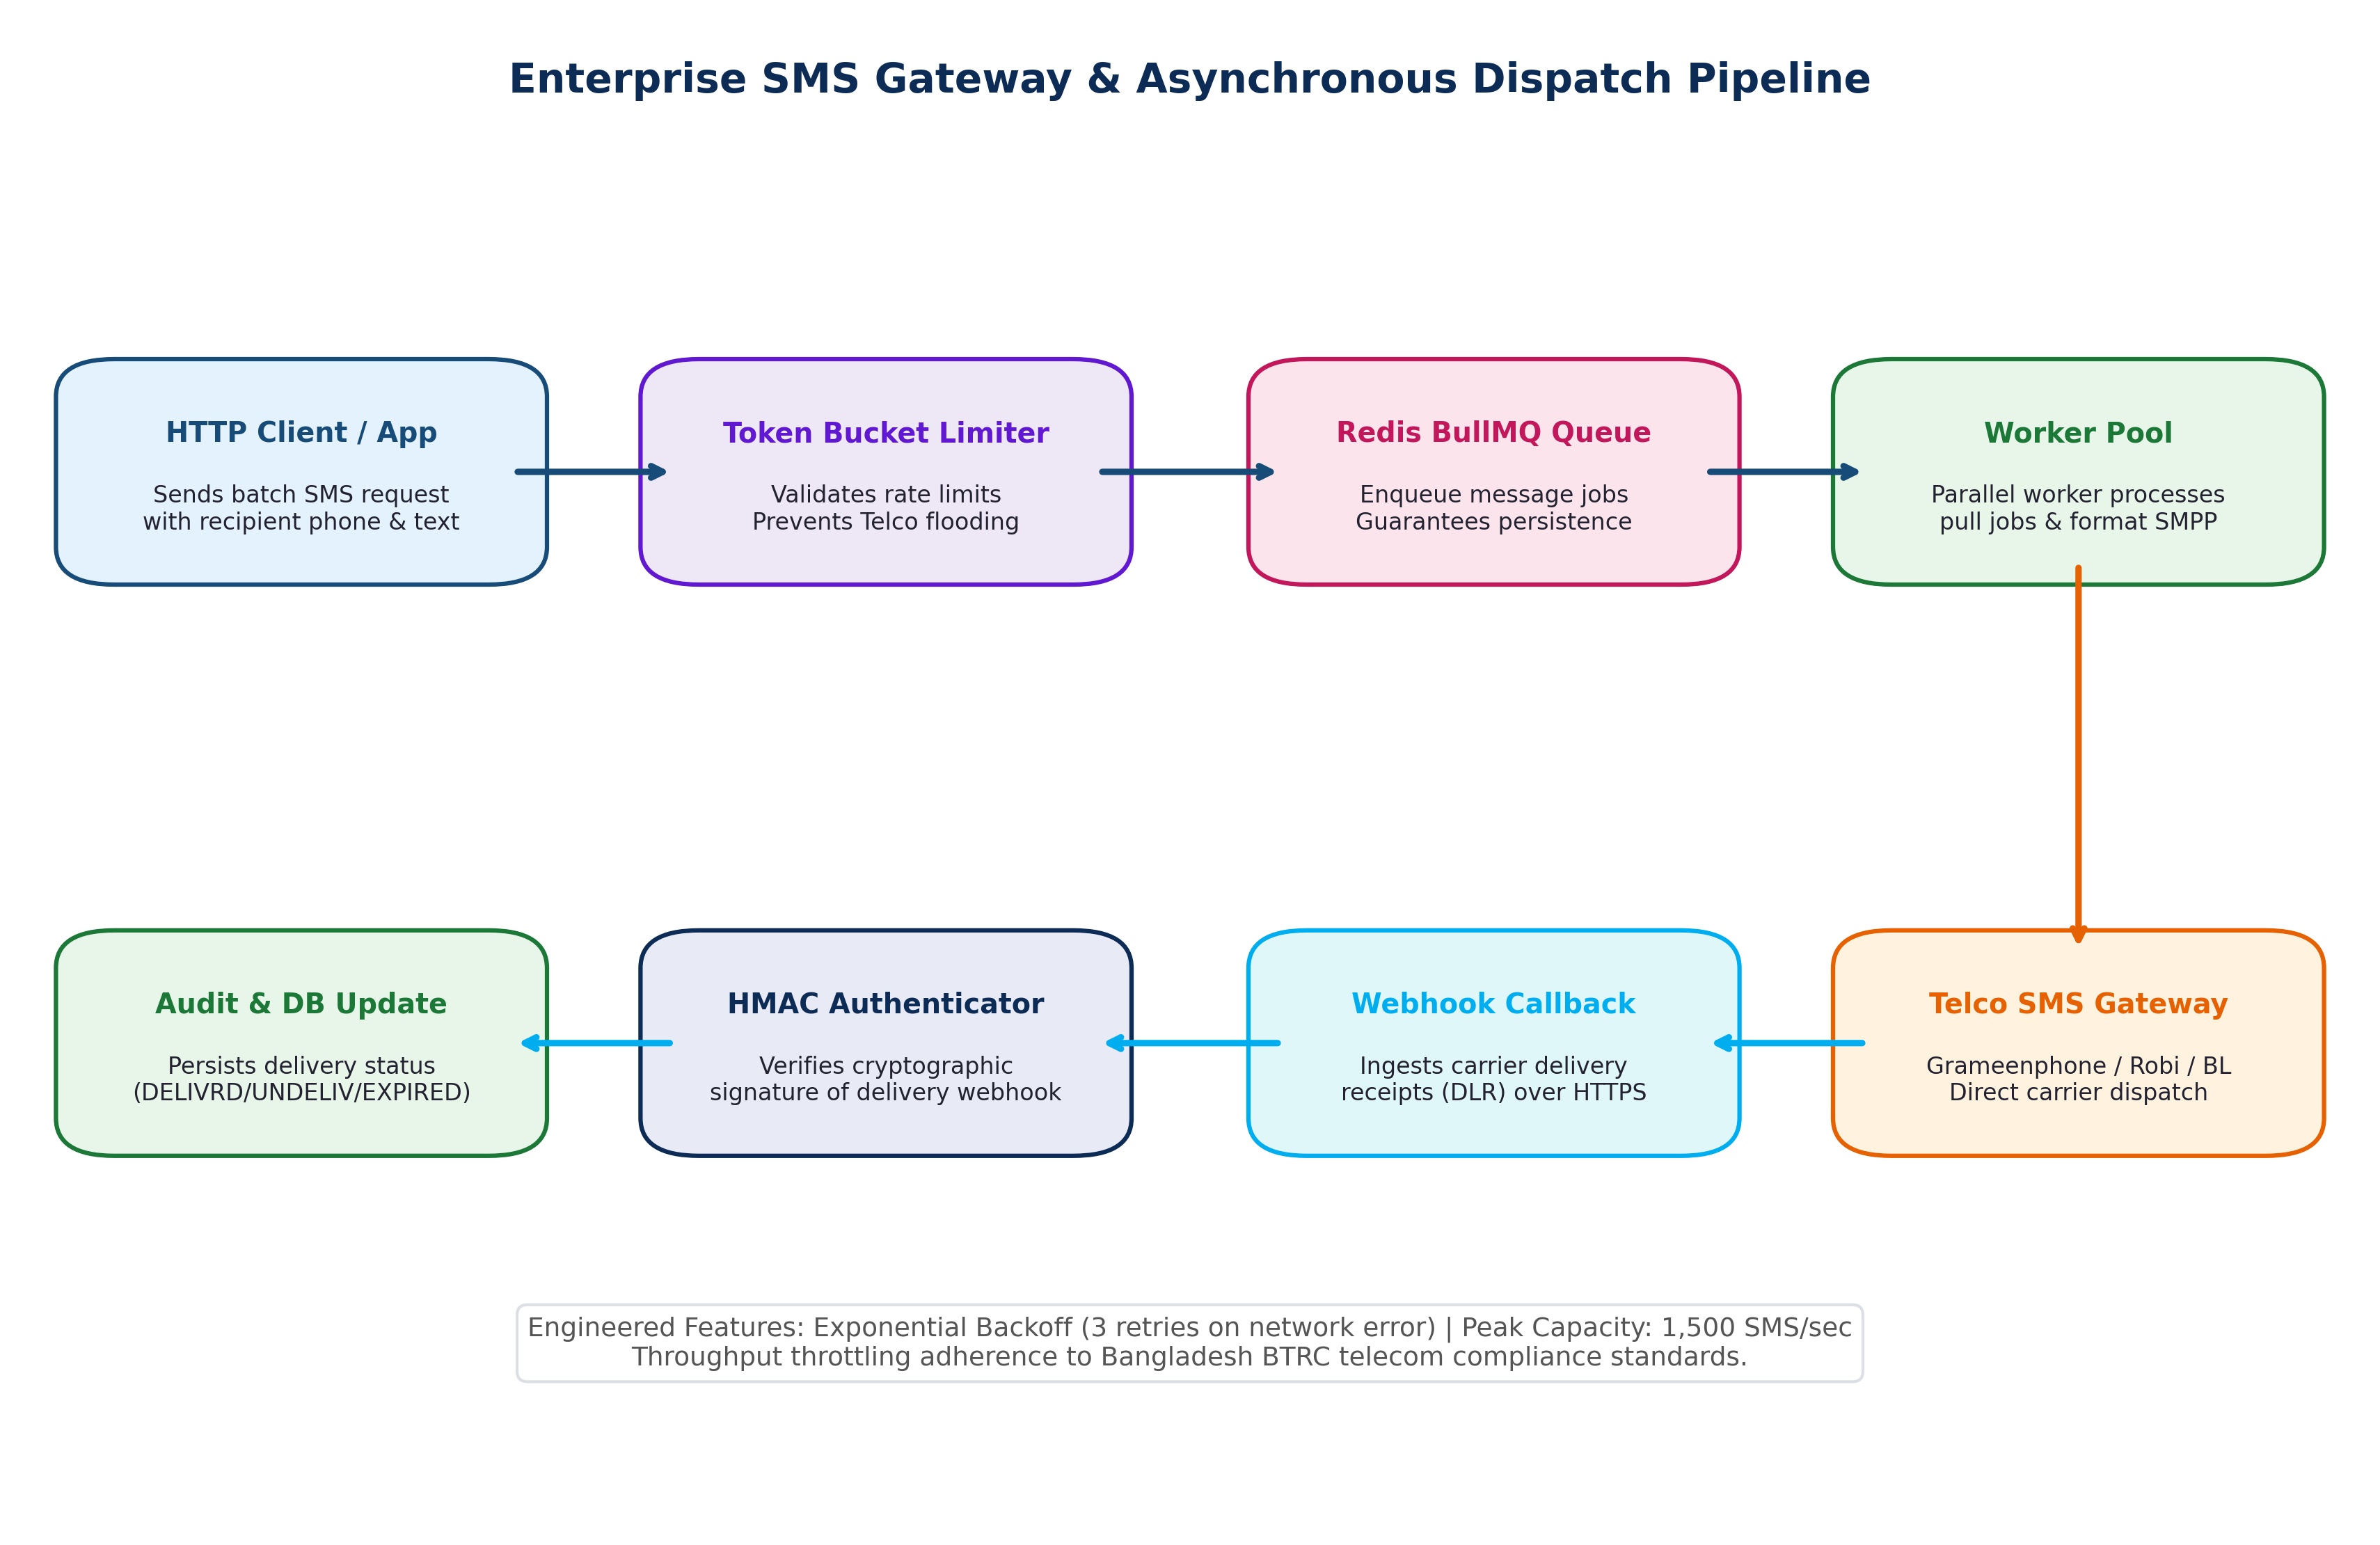
\includegraphics[width=0.95\textwidth]{figures/sms_gateway_pipeline.png}
    \caption{Enterprise SMS Gateway and Asynchronous Dispatch Pipeline.}
    \label{fig:sms_gateway_pipeline}
\end{figure}

\subsection{Pipeline Mechanics}
\begin{enumerate}
    \item \textbf{Ingestion \& Rate Limiting:} Clients initiate single or bulk SMS dispatch requests via HTTPS. The request passes through an in-memory \textbf{Token Bucket Rate Limiter} implemented via Redis atomic operations, guaranteeing that inbound client traffic does not overwhelm internal capacity.
    \item \textbf{Queue Decoupling (Producer):} The API service acts as a producer, persisting initial message metadata into PostgreSQL and enqueuing jobs into the \textbf{BullMQ Redis Queue}. The HTTP connection immediately terminates with an HTTP \texttt{202 Accepted} response and tracking UUID, freeing the client from carrier latency.
    \item \textbf{Parallel Worker Pool (Consumer):} Clustered BullMQ worker processes continuously pull pending jobs from Redis. Workers format the payload to carrier-specific SMPP or HTTP protocols, execute telco routing, and dispatch messages across direct interconnects with Bangladesh operators (Grameenphone, Robi, Banglalink, Teletalk).
    \item \textbf{Retry with Exponential Backoff:} If a telecom carrier endpoint returns a transient network timeout or HTTP 5xx error, BullMQ automatically schedules retries using an exponential backoff formula:
    \begin{equation}
        T_{\text{wait}} = T_{\text{base}} \times 2^{\text{attempt}} + \text{jitter}
    \end{equation}
    preventing thundering herd problems against carrier gateways.
    \item \textbf{Webhook Ingestion \& Cryptographic Verification:} When carriers deliver messages to handsets, they dispatch an asynchronous Delivery Receipt (DLR) webhook to Digicon. An HMAC-SHA256 signature guard verifies that the webhook genuinely originated from the carrier, after which the delivery state is updated in PostgreSQL.
\end{enumerate}

\section{JWT Authentication and Role-Based Access Control Flow}
\label{sec:arch_jwt_flow}

To satisfy non-functional security requirements, authentication and authorization are unified into a stateless, cryptographically enforced pipeline. Figure~\ref{fig:jwt_auth_workflow} illustrates the sequence of interactions governing access.

\begin{figure}[htbp]
    \centering
    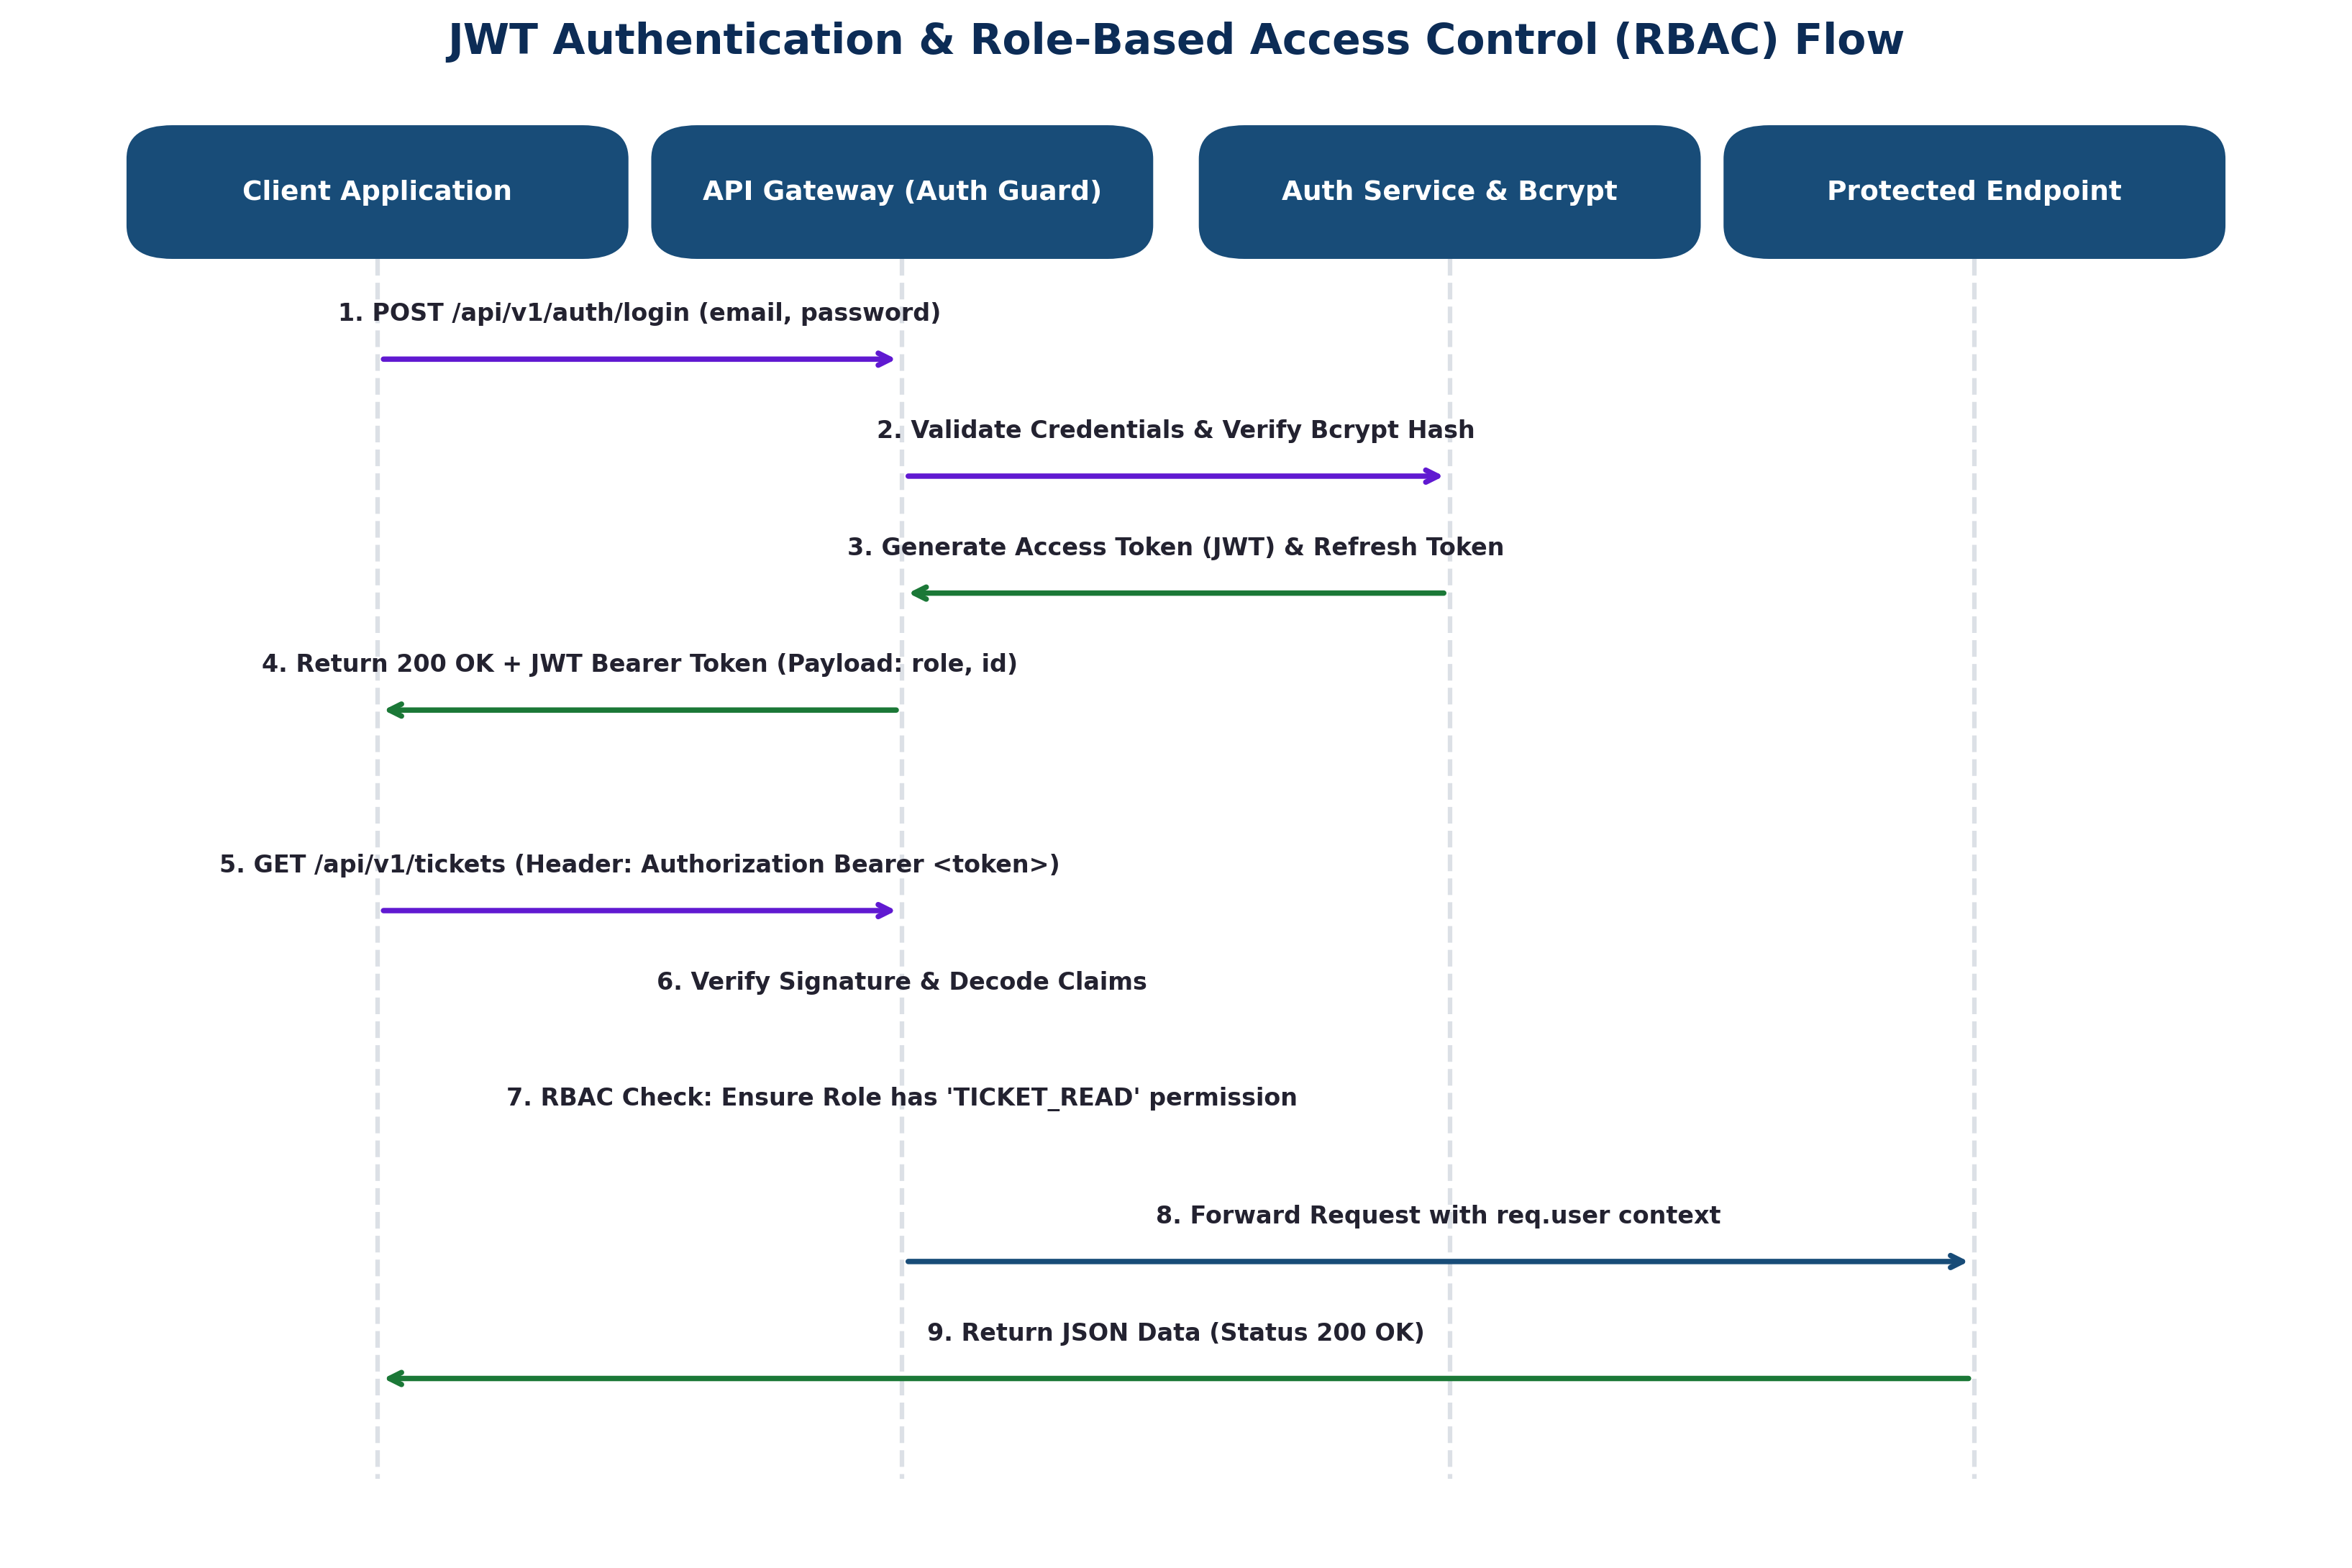
\includegraphics[width=0.95\textwidth]{figures/jwt_auth_workflow.png}
    \caption{JWT Authentication and Role-Based Access Control (RBAC) Flow.}
    \label{fig:jwt_auth_workflow}
\end{figure}

The authentication lifecycle proceeds as follows:
\begin{enumerate}
    \item \textbf{Credential Verification:} The client submits an email and password to \texttt{POST /api/v1/auth/login}. The Auth Service retrieves the user record from PostgreSQL and verifies the Bcrypt hash.
    \item \textbf{Token Minting:} Upon successful authentication, the server mints a short-lived Access Token (JWT) containing the user's UUID, assigned role, and permissions, along with a cryptographically random Refresh Token persisted in Redis.
    \item \textbf{Protected Endpoint Invocation:} Subsequent requests to protected routes (e.g., \texttt{GET /api/v1/tickets}) supply the JWT within the standard HTTP \texttt{Authorization: Bearer <token>} header.
    \item \textbf{Stateless Signature Verification:} The API Gateway Guard verifies the token's cryptographic signature using a shared secret key without querying the database, eliminating authentication bottlenecks.
    \item \textbf{RBAC Permission Evaluation:} An authorization guard inspects the decoded role claims against the endpoint's permission decorator. If the role possesses the required permission (e.g., \texttt{TICKET\_READ}), the request proceeds to controller execution; otherwise, an immediate HTTP \texttt{403 Forbidden} error is returned.
\end{enumerate}

\section{DevOps and Continuous Deployment Pipeline}
\label{sec:arch_devops}

To maintain engineering consistency across development, staging, and production environments, Digicon utilizes a structured DevOps pipeline. Figure~\ref{fig:ci_cd_docker_pipeline} depicts the continuous integration and deployment workflow.

\begin{figure}[htbp]
    \centering
    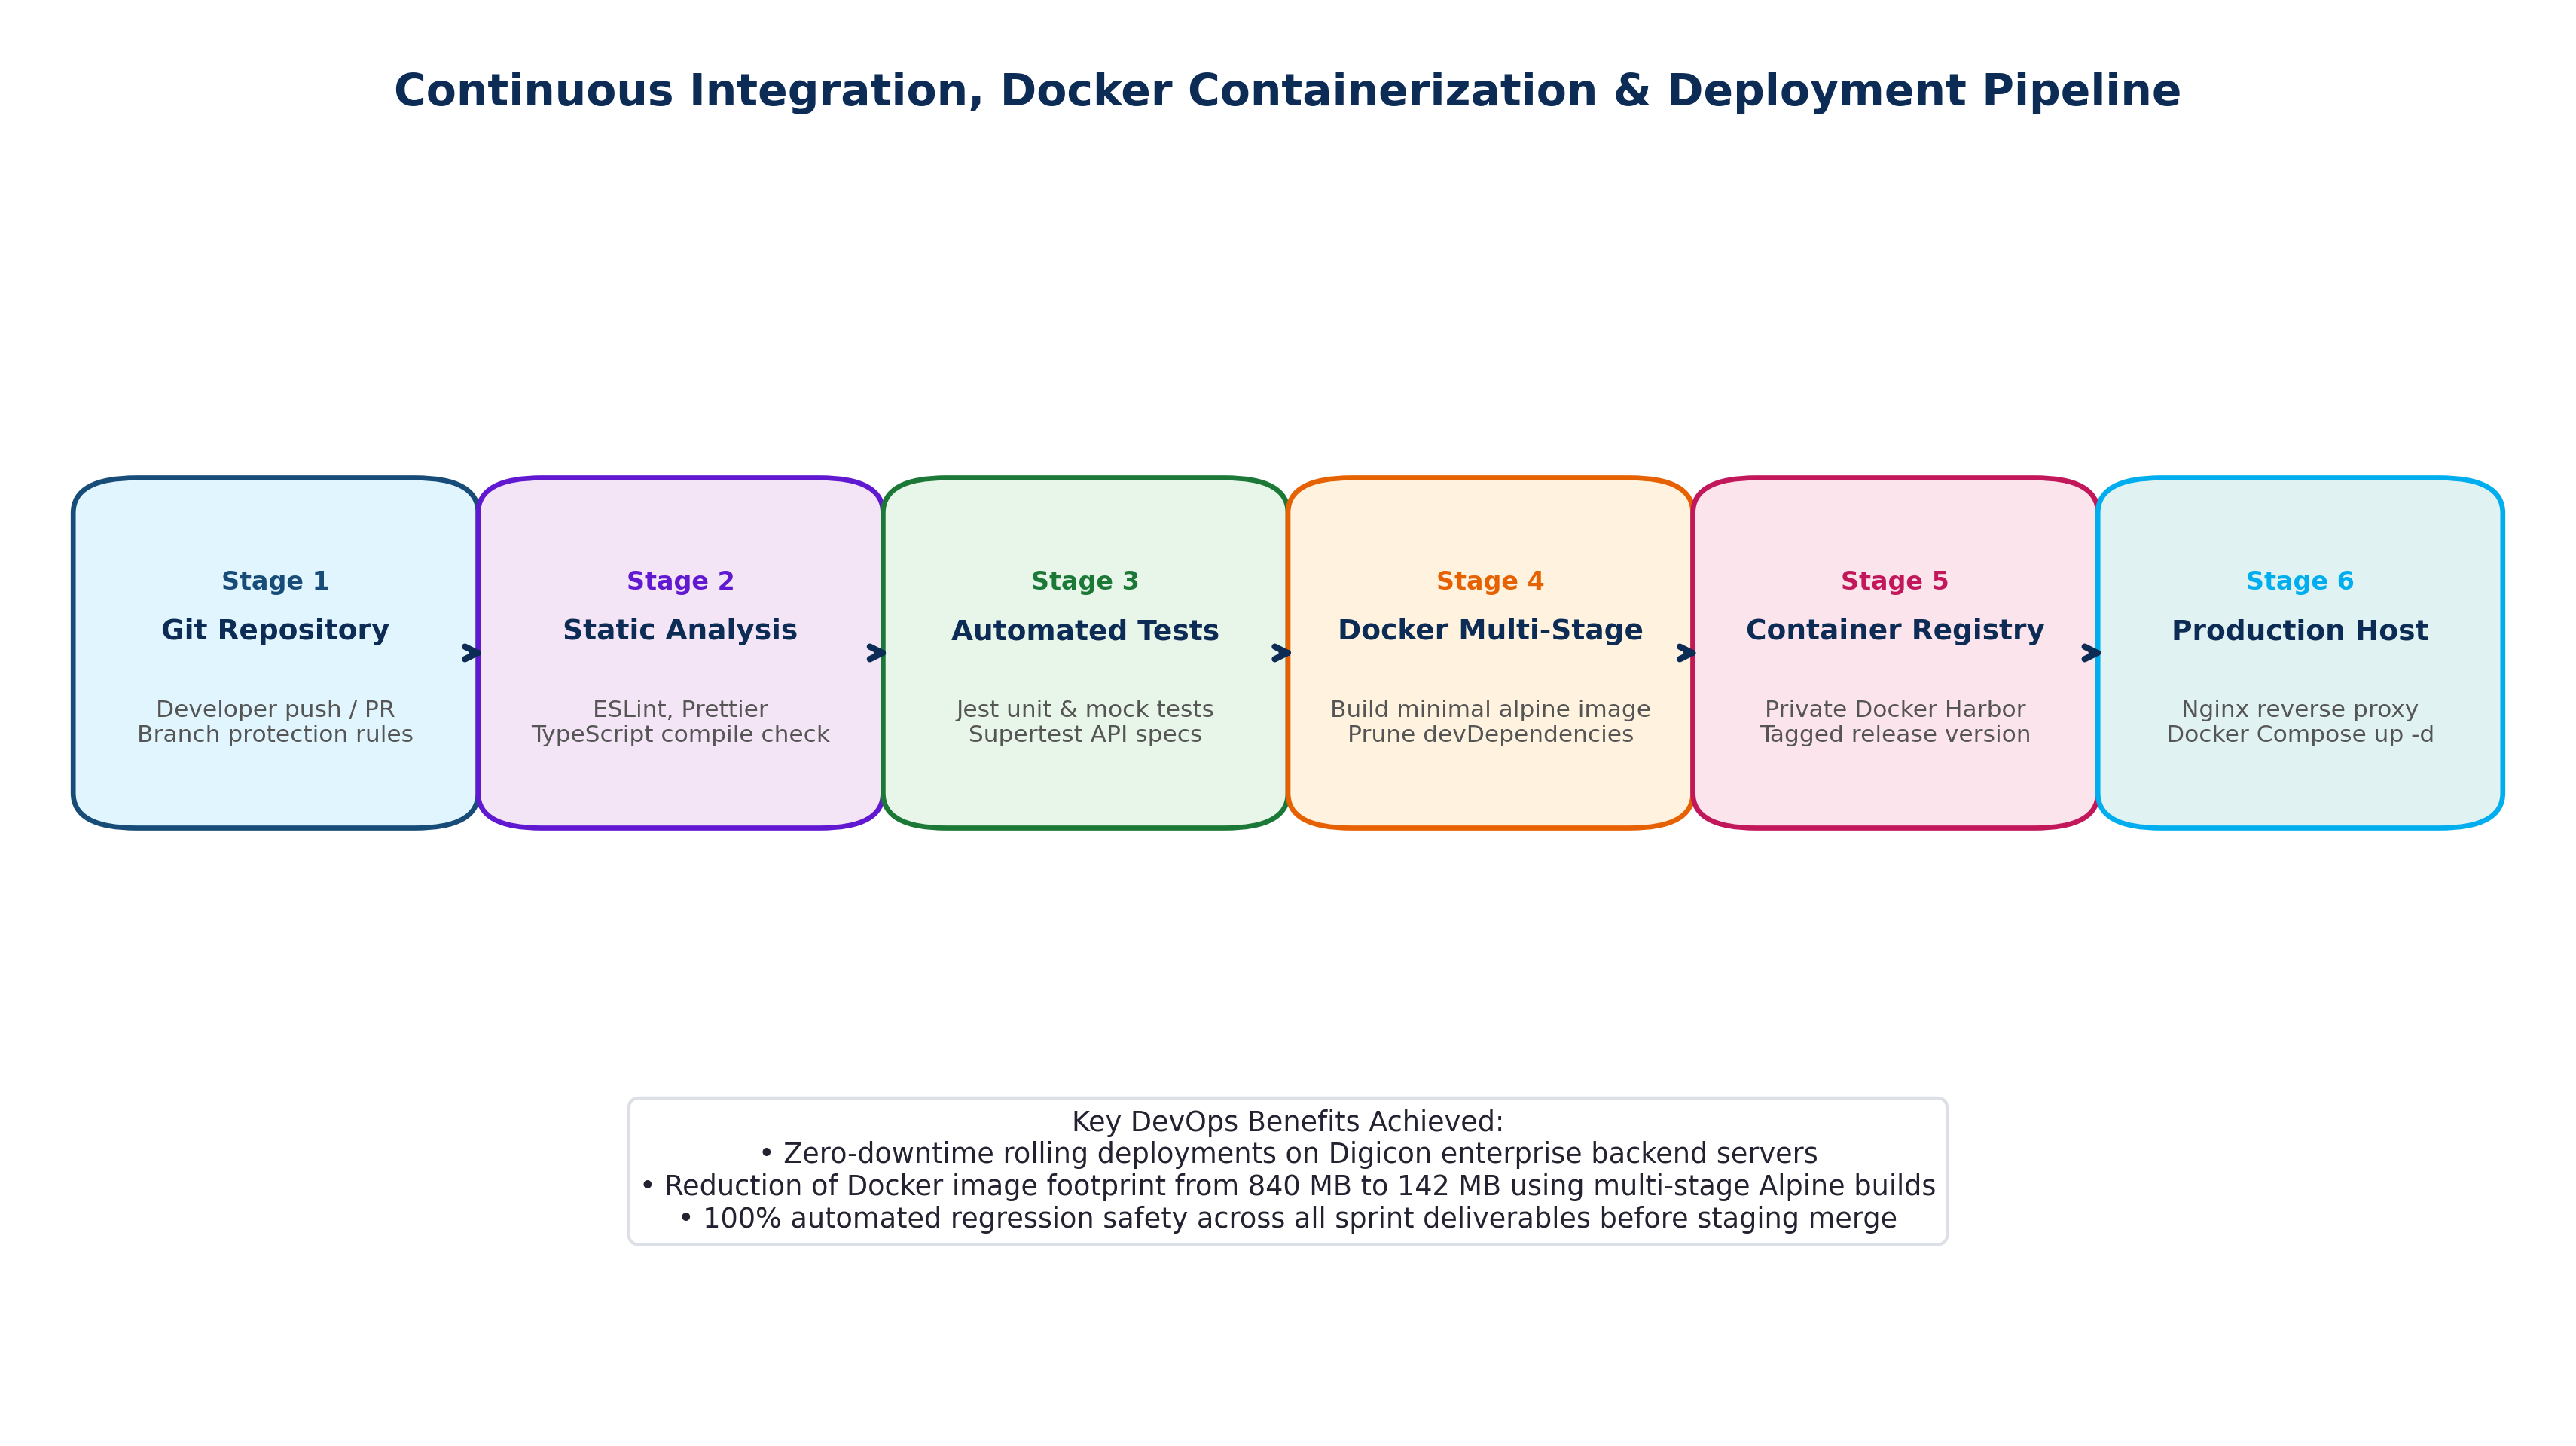
\includegraphics[width=0.95\textwidth]{figures/ci_cd_docker_pipeline.png}
    \caption{Continuous Integration, Docker Containerization and Deployment Pipeline.}
    \label{fig:ci_cd_docker_pipeline}
\end{figure}

The pipeline enforces rigorous quality gates:
\begin{itemize}
    \item \textbf{Stage 1: Git Version Control:} Developers push feature branches and submit Pull Requests (PR) against the primary development branch.
    \item \textbf{Stage 2: Static Analysis:} Automated Git hooks execute ESLint and Prettier formatting checks, followed by TypeScript strict compilation checks.
    \item \textbf{Stage 3: Automated Testing:} The CI pipeline executes comprehensive Jest unit tests and Supertest API specifications. Pull Requests cannot be merged if any test fails or if coverage drops below the 80\% threshold.
    \item \textbf{Stage 4: Multi-Stage Docker Build:} A minimal, production-optimized Alpine Linux Docker image is constructed, discarding compilation tools and \texttt{devDependencies}.
    \item \textbf{Stage 5: Container Registry Storage:} The verified image is tagged with the semantic Git release version and pushed to Digicon's private Docker registry.
    \item \textbf{Stage 6: Zero-Downtime Deployment:} Production host servers pull the updated container image and execute a rolling container restart behind Nginx load balancers without dropping active user connections.
\end{itemize}
